% !TeX program = xelatex
\ifdefined\BookMaster\else
\documentclass[11pt,oneside]{article}
% !TeX program = xelatex
\usepackage[b5paper,left=22mm,right=22mm,top=20mm,bottom=22mm,footskip=11mm]{geometry}
\usepackage{fontspec}
\setmainfont{TeX Gyre Termes}
\setsansfont{TeX Gyre Heros}
\usepackage{amsmath,amssymb,mathtools,amsthm}
\renewcommand{\cdots}{\mathinner{\cdotp\cdotp\cdotp}}
\usepackage{graphicx,adjustbox,array,booktabs,longtable,multirow,enumitem,changepage,needspace}
\usepackage[table]{xcolor}
\usepackage{fancyhdr}
\raggedbottom
\interfootnotelinepenalty=10000
\newcommand{\BookFootnote}[2]{\begingroup\renewcommand{\thefootnote}{\fnsymbol{footnote}}\footnote[#1]{#2}\endgroup}
\newcommand{\BookFootnoteMark}[1]{\begingroup\renewcommand{\thefootnote}{\fnsymbol{footnote}}\footnotemark[#1]\endgroup}
\newcommand{\BookFootnoteText}[2]{\begingroup\renewcommand{\thefootnote}{\fnsymbol{footnote}}\footnotetext[#1]{#2}\endgroup}
\newenvironment{BookFloat}[1]{\par\addvspace{.6\baselineskip}\noindent\def\BookFloatID{#1}\begin{minipage}{\linewidth}\phantomsection\label{bookfloat:#1:start}}{\phantomsection\label{bookfloat:\BookFloatID:end}\end{minipage}\par\addvspace{.6\baselineskip}}

\usepackage[unicode,hidelinks]{hyperref}
\pagestyle{fancy}
\fancyhf{}
\newcommand{\BookFooter}{}
\fancyfoot[L]{\parbox[b]{\dimexpr\textwidth-15mm}{\footnotesize\BookFooter}}
\fancyfoot[R]{\footnotesize\thepage}
\renewcommand{\headrulewidth}{0pt}
\renewcommand{\footrulewidth}{0pt}
\setlength{\parindent}{0pt}
\setlength{\parskip}{0.2em}
\setlength{\emergencystretch}{3em}
\setlist{nosep,leftmargin=1.7em,labelsep=.65em}
\newif\ifBookNarrative
\BookNarrativetrue
\newenvironment{BookBody}{\setlength{\parindent}{0pt}}{}
\newcommand{\BookStatement}[1]{\par\addvspace{.6\baselineskip}\noindent #1\enspace\ignorespaces}
\newcommand{\BookLabel}[1]{\par\addvspace{.6\baselineskip}\needspace{3\baselineskip}\noindent\textbf{#1}\quad\ignorespaces}
\newcommand{\BookHeading}[1]{\par\addvspace{\baselineskip}\needspace{4\baselineskip}\noindent{\large\bfseries #1}\par\medskip}
\newcommand{\BookSubheading}[1]{\par\addvspace{.7\baselineskip}\needspace{3\baselineskip}\noindent{\bfseries #1}\par\smallskip}
\newcommand{\BookTextHeading}[1]{\par\addvspace{.7\baselineskip}\needspace{3\baselineskip}\noindent #1\par\smallskip}
\newcommand{\BookSectionTitle}[2]{\par\addvspace{1.2\baselineskip}\needspace{5\baselineskip}\noindent\colorbox{gray!25}{\sffamily\bfseries\small SECTION #1}\quad{\large\bfseries #2}\par\medskip}
\newcommand{\BookExerciseTitle}[1]{\par\addvspace{\baselineskip}\needspace{4\baselineskip}\noindent{\color{gray}\rule{1.5mm}{1.5mm}}\enspace{\large\bfseries Exercises #1}\par\medskip}
\newcommand{\BookBullet}[1]{\begin{list}{\textbullet}{\setlength{\leftmargin}{1.7em}\setlength{\labelwidth}{1em}\setlength{\labelsep}{.7em}\setlength{\topsep}{0pt}\setlength{\parsep}{0pt}\setlength{\itemsep}{0pt}}\item #1\end{list}}
\newcommand{\BookExercise}[2]{\begin{list}{\textbf{#1}}{\setlength{\leftmargin}{2.2em}\setlength{\labelwidth}{1.5em}\setlength{\labelsep}{.7em}\setlength{\topsep}{.15em}\setlength{\parsep}{0pt}\setlength{\itemsep}{0pt}}\item #2\end{list}}
\newcommand{\BookEnd}[1]{\unskip\nobreak\hfill\ensuremath{#1}}
\newcommand{\BookSource}[2]{\phantomsection\label{sourcepage:#1}} % Source-page anchors, retained through reflow.
\usepackage{multicol}
\usepackage{tikz}
\newcommand{\BookPartEntry}[2]{\par\noindent\makebox[17mm][l]{\bfseries Section #1}#2\par}
\newcommand{\BookPartTitle}[3]{\par\bigskip\noindent\begin{tikzpicture}\node[anchor=north west,inner sep=0pt,outer sep=0pt] (bookpart) at (0,0) {\begin{minipage}{\dimexpr\linewidth-.5pt}\hspace*{26mm}\begin{minipage}[t]{\dimexpr\linewidth-26mm}\begin{adjustbox}{max width=\linewidth}{\fontsize{20}{24}\selectfont\bfseries #2}\end{adjustbox}\par\vspace{6mm}\hrule\vspace{6mm}{\sffamily\footnotesize\setlength{\parskip}{.3em}#3}\vspace{3mm}\end{minipage}\end{minipage}};\path[shade,top color=gray!60,bottom color=white] (0,0) rectangle ([xshift=24mm]bookpart.south west);\node[anchor=north,font=\sffamily\bfseries\small] at (12mm,-2mm) {PART};\node[anchor=north,font=\sffamily\bfseries\Huge] at (12mm,-7mm) {#1};\end{tikzpicture}\par\bigskip}
\newsavebox{\BookMathBox}
\makeatletter
\newcommand{\BookInline}[1]{\leavevmode\hskip0pt\relax\begingroup\in@{\begin}{#1}\ifin@\sbox{\BookMathBox}{\(#1\)}\ifdim\wd\BookMathBox>\dimexpr\linewidth-1em\relax\resizebox{\dimexpr\linewidth-1em\relax}{!}{\usebox{\BookMathBox}}\else\(#1\)\fi\else\in@{\left}{#1}\ifin@\sbox{\BookMathBox}{\(#1\)}\ifdim\wd\BookMathBox>\dimexpr\linewidth-1em\relax\resizebox{\dimexpr\linewidth-1em\relax}{!}{\usebox{\BookMathBox}}\else\(#1\)\fi\else\(#1\)\fi\fi\endgroup\hskip0pt\relax}
\makeatother
\DeclareMathOperator{\Aut}{Aut}
\DeclareMathOperator{\End}{End}
\DeclareMathOperator{\Hom}{Hom}
\DeclareMathOperator{\GF}{GF}
\DeclareMathOperator{\irr}{irr}
\DeclareMathOperator{\lt}{lt}
\DeclareMathOperator{\lp}{lp}
\providecommand{\textcircled}[1]{\textnormal{(#1)}}

\begin{document}
\fi
\renewcommand{\BookFooter}{Section 7 Generating Sets and Cayley Digraphs}
\pdfbookmark[0]{Section 7 Generating Sets and Cayley Digraphs}{07_generating_sets_and_cayley_digraphs}
\ifdefined\BookMaster\else\setcounter{page}{70}\fi
% Source PDF page 87; original printed page 70
\BookSource{87}{70}
\BookNarrativetrue

\begin{BookBody}

\BookSectionTitle{7}{Generating Sets and Cayley Digraphs}

\noindent Let \BookInline{G} be a group, and let \BookInline{a\in G.} We have described the cyclic subgroup \BookInline{\langle a\rangle } of \BookInline{G,\allowbreak } which is the smallest subgroup of \BookInline{G} that contains the element \BookInline{a.} Suppose we want to find as small a subgroup as possible that contains both \BookInline{a} and \BookInline{b} for another element \BookInline{b} in \BookInline{G.} By Theorem 5.19, we see that any subgroup containing \BookInline{a} and \BookInline{b} must contain \BookInline{a^{n}} and \BookInline{b^{m}} for all \BookInline{m,\allowbreak n\in \mathbb{Z},\allowbreak } and consequently must contain all finite products of such powers of \BookInline{a} and \BookInline{b.} For example, such an expression might be \BookInline{a^{2}b^{4}a^{- 3}b^{2}a^{5}.} Note that we cannot “simplify” this expression by writing first all powers of \BookInline{a} followed by the powers of \BookInline{b,\allowbreak } since \BookInline{G} may not be abelian. However, products of such expressions are again expressions of the same type. Furthermore\BookInline{,\allowbreak e= a^{0}} and the inverse of such an expression is again of the same type. For example, the inverse of \BookInline{a^{2}b^{4}a^{- 3}b^{2}a^{5}} is \BookInline{a^{- 5}b^{- 2}a^{3}b^{- 4}a^{- 2}.} By Theorem 5.12, this shows that all such products of integral powers of \BookInline{a} and \BookInline{b} form a subgroup of \BookInline{G,\allowbreak } which surely must be the smallest subgroup containing both \BookInline{a} and \BookInline{b.} We call \BookInline{a} and \BookInline{b} \textbf{generators} of this subgroup. If this subgroup should be all of \BookInline{G,\allowbreak } then we say that \BookInline{\{a,\allowbreak b\}} \textbf{generates} \BookInline{G.} Of course, there is nothing sacred about taking just two elements \BookInline{a,\allowbreak b\in G.} We could have made similar arguments for three, four, or any number of elements of \BookInline{G,\allowbreak } as long as we take only finite products of their integral powers.

\BookLabel{7.1 Example} As we have seen, the dihedral group is generated by \BookInline{\{\mu,\allowbreak \rho \}} since every element in \BookInline{D_{n}} can be written in the form \BookInline{\rho ^{k}} or \BookInline{\mu \rho ^{k}} for \BookInline{0\leq k<n.} Also\BookInline{,\allowbreak \{\mu,\allowbreak \mu \rho \}} generates \BookInline{D_{n}} since \BookInline{\rho = \mu (\mu \rho ),\allowbreak } so any element in the dihedral group can also be written as a product of copies of \BookInline{\mu } and \BookInline{\mu \rho.} It is interesting to note that both \BookInline{\mu } and \BookInline{\mu \rho } have order 2, while in the generating set \BookInline{\{\mu,\allowbreak \rho \}} one element has order 2, but the other has order \BookInline{n.}\BookEnd{\blacktriangle}

\BookLabel{7.2 Example} The Klein 4-group \BookInline{V= \{e,\allowbreak a,\allowbreak b,\allowbreak c\}} of Example 5.7 is generated by \BookInline{\{a,\allowbreak b\}} since \BookInline{ab= c.} It is also generated by \BookInline{\{a,\allowbreak c\},\allowbreak \{b,\allowbreak c\},\allowbreak } and \BookInline{\{a,\allowbreak b,\allowbreak c\}.} If a group \BookInline{G} is generated by a subset \BookInline{S,\allowbreak } then every subset of \BookInline{G} containing \BookInline{S} generates \BookInline{G.}\BookEnd{\blacktriangle}

\BookLabel{7.3 Example} The group \BookInline{\mathbb{Z}_{6}} is generated by \BookInline{\{1\}} and \BookInline{\{5\}.} It is also generated by \BookInline{\{2,\allowbreak 3\}} since \BookInline{2+ 3= 5,\allowbreak } so that any subgroup containing 2 and 3 must contain 5 and must therefore be \BookInline{\mathbb{Z}_{6}.} It is also generated by \BookInline{\{3,\allowbreak 4\},\allowbreak \{2,\allowbreak 3,\allowbreak 4\},\allowbreak \{1,\allowbreak 3\},\allowbreak } and \BookInline{\{3,\allowbreak 5\},\allowbreak } but it is not generated by \BookInline{\{2,\allowbreak 4\}} since \BookInline{\langle 2\rangle = \{0,\allowbreak 2,\allowbreak 4\}} contains 2 and \BookInline{4.}\BookEnd{\blacktriangle}

\end{BookBody}

% Source PDF page 88; original printed page 71
\BookSource{88}{71}
\BookNarrativetrue

\begin{BookBody}

We have given an intuitive explanation of the subgroup of a group \BookInline{G} generated by a subset of \BookInline{G.} What follows is a detailed exposition of the same idea approached in another way, namely via intersections of subgroups. After we get an intuitive grasp of a concept, it is nice to try to write it up as neatly as possible. We give a set-theoretic definition and generalize a theorem that was in Exercise 61 of Section 5.

\BookLabel{7.4 Definition} Let \BookInline{\{S_{i}\mid i\in I\}} be a collection of sets. Here \BookInline{I} may be any set of indices. The\textbf{ intersection} \BookInline{\cap _{i\in I}S_{i}} \textbf{of the sets} \BookInline{S_{i}} is the set of all elements that are in all the sets \BookInline{S_{i};} that is,

\begin{center}\begin{adjustbox}{max width=\linewidth}\BookInline{\displaystyle \bigcap _ { i \in I } S _ { i } = \{ x   |   x \in S _ { i } { \mathrm { ~ f o r ~ a l l ~ } } i \in I \} .}\end{adjustbox}\end{center}

\noindent If \BookInline{I} is finite\BookInline{,\allowbreak I= \{1,\allowbreak 2,\allowbreak...,\allowbreak n\},\allowbreak } we may denote \BookInline{\cap _{i\in I}S_{i}} by

\begin{center}\begin{adjustbox}{max width=\linewidth}\BookInline{\displaystyle S_{1}\cap S_{2}\cap \cdots \cap S_{n}.}\end{adjustbox}\end{center} \BookEnd{\blacksquare}

\BookLabel{7.5 Theorem} For any group \BookInline{G} and any nonempty collection of subgroups \BookInline{\{H_{i}\leq G\mid i\in I\},\allowbreak } the intersection of all the subgroups \BookInline{H_{i},\allowbreak \cap _{i\in I}H_{i},\allowbreak } is also a subgroup of \BookInline{G.}

\BookLabel{\textit{Proof}} Let us show closure. Let \BookInline{a\in \cap _{i\in I}H_{i}} and \BookInline{b\in \cap _{i\in I}H_{i},\allowbreak } so that \BookInline{a\in H_{i}} for all \BookInline{i\in I} and \BookInline{b\in H_{i}} for all \BookInline{i\in I.} Then \BookInline{ab\in H_{i}} for all \BookInline{i\in I,\allowbreak } since \BookInline{H_{i}} is a group. Thus \BookInline{ab\in \cap _{i\in I}H_{i}.} Since \BookInline{H_{i}} is a subgroup for all \BookInline{i\in I,\allowbreak } we have \BookInline{e\in H_{i}} for all \BookInline{i\in I,\allowbreak } and hence \BookInline{e\in \cap _{i\in I}H_{i}.}

Finally, for \BookInline{a\in \cap _{i\in I}H_{i},\allowbreak } we have \BookInline{a\in H_{i}} for all \BookInline{i\in I,\allowbreak } so \BookInline{a^{- 1}\in H_{i}} for all \BookInline{i\in I,\allowbreak } which implies that \BookInline{a^{- 1}\in \cap _{i\in I}H_{i}.}\BookEnd{\blacklozenge}

Let \BookInline{G} be a group and let \BookInline{a_{i}\in G} for \BookInline{i\in I.} There is at least one subgroup of \BookInline{G} containing all the elements \BookInline{a_{i}} for \BookInline{i\in I,\allowbreak } namely \BookInline{G} is itself. Theorem 7.5 assures us that if we take the intersection of all subgroups of \BookInline{G} containing all \BookInline{a_{i}} for \BookInline{i\in I,\allowbreak } we will obtain a subgroup \BookInline{H} of \BookInline{G.} This subgroup \BookInline{H} is the smallest subgroup of \BookInline{G} containing all the \BookInline{a_{i}} for \BookInline{i\in I.}

\BookLabel{7.6 Definition} Let \BookInline{G} be a group and let \BookInline{a_{i}\in G} for \BookInline{i\in I.} The smallest subgroup of \BookInline{G} containing \BookInline{\{a_{i}\mid i\in } \BookInline{I\}} is the\textbf{ subgroup generated by} \BookInline{\{a_{i}\mid i\in I\}.} If this subgroup is all of \BookInline{G,\allowbreak } then \BookInline{\{a_{i}\mid i\in } \BookInline{I\}} \textbf{generates} \BookInline{G} and the \BookInline{a_{i}} are\textbf{ generators of} \BookInline{G.} If there is a finite set \BookInline{\{a_{i}\mid i\in I\}} that generates \BookInline{G,\allowbreak } then \BookInline{G} is\textbf{ finitely generated}\BookInline{.}\BookEnd{\blacksquare}

Note that this definition is consistent with our previous definition of a generator for a cyclic group. Note also that the statement \BookInline{a} \textit{is} \BookInline{a} \textit{generator of} \BookInline{G} may mean either that \BookInline{G= \langle a\rangle } or that \BookInline{a} is a member of a subset of \BookInline{G} that generates \BookInline{G.} The context in which the statement is made should indicate which is intended. Our next theorem gives the structural insight into the subgroup of \BookInline{G} generated by \BookInline{\{a_{i}\mid i\in I\}} that we discussed for two generators before Example 7.1.

\BookLabel{7.7 Theorem} If \BookInline{G} is a group and \BookInline{a_{i}\in G} for \BookInline{i\in I\neq \phi,\allowbreak } then the subgroup \BookInline{H} of \BookInline{G} generated by \BookInline{\{a_{i}\mid i\in } \BookInline{I\}} has as elements precisely those elements of \BookInline{G} that are finite products of integral powers of the \BookInline{a_{i},\allowbreak } where powers of a fixed \BookInline{a_{i}} may occur several times in the product.

\BookLabel{\textit{Proof}} Let \BookInline{K} denote the set of all finite products of integral powers of the \BookInline{a_{i}.} Then \BookInline{K\subseteq H.} We need only observe that \BookInline{K} is a subgroup and then, since \BookInline{H} is the smallest subgroup containing \BookInline{a_{i}} for \BookInline{i\in I,\allowbreak } we will be done. Observe that a product of elements in \BookInline{K} is again in \BookInline{K.} Since \BookInline{(a_{i})^{0}= e,\allowbreak } we have \BookInline{e\in K.} For every element \BookInline{k} in \BookInline{K,\allowbreak } if we form from the product giving \BookInline{k} a new product with the order of the \BookInline{a_{i}} reversed and the opposite sign on all exponents, we have \BookInline{k^{- 1},\allowbreak } which is thus in \BookInline{K.} For example,

\begin{center}\begin{adjustbox}{max width=\linewidth}\BookInline{\displaystyle \Big[(a_{1})^{3}(a_{2})^{2}(a_{1})^{- 7}\Big]^{- 1}= (a_{1})^{7}(a_{2})^{- 2}(a_{1})^{- 3},\allowbreak }\end{adjustbox}\end{center}

\noindent which is again in \BookInline{K.} \BookEnd{\blacklozenge}

\end{BookBody}

% Source PDF page 89; original printed page 72
\BookSource{89}{72}
\BookNarrativetrue

\begin{BookBody}

\BookLabel{7.8 Example} Recall that the dihedral group \BookInline{D_{n}} consists of permutations of \BookInline{\mathbb{Z}_{n}} that map edges to edges in the regular \BookInline{n-}gon \BookInline{P_{n}.} In disjoint cycle notation, \BookInline{\rho=(0,1,2,3,\ldots,n-1)} and \BookInline{\mu=(1,n-1)(2,n-2)\cdots\left(\frac{n-1}{2},\frac{n+1}{2}\right)} if \BookInline{n} is odd, and \BookInline{\mu=(1,n-1)(2,n-2)\cdots\left(\frac{n-2}{2},\frac{n+2}{2}\right)} if \BookInline{n} is even. Since \BookInline{\mu ^{2}= \iota } and \BookInline{\rho ^{n}= \iota } any product of integer powers of \BookInline{\mu } and \BookInline{\rho } can be rewritten to only have powers of 0 or 1 for \BookInline{\mu } and powers of \BookInline{0,\allowbreak 1,\allowbreak 2,\allowbreak 3,\allowbreak...n- 1} for \BookInline{\rho.} Furthermore, the relation \BookInline{\rho \mu = \mu \rho ^{n- 1}} allows us to move all the powers of \BookInline{\mu } to the left and all the powers of \BookInline{\rho } to the right, being careful to replace \BookInline{\rho } with \BookInline{\rho ^{n- 1}} each time we move a \BookInline{\mu } past a \BookInline{\rho.} So in the case of \BookInline{n= 6,\allowbreak }

\begin{center}\begin{adjustbox}{max width=\linewidth}\BookInline{\displaystyle \rho ^{8}\mu ^{9}= \rho ^{2}\mu = \rho \mu \rho ^{5}= \mu \rho ^{5}\rho ^{5}= \mu \rho ^{4}.}\end{adjustbox}\end{center}

\noindent Thus the subgroup of \BookInline{S_{\mathbb{Z}_{n}}} generated by \BookInline{\mu } and \BookInline{\rho } is the set

\begin{center}\begin{adjustbox}{max width=\linewidth}\BookInline{\displaystyle \{\iota ,\allowbreak \rho ,\allowbreak \rho ^{2},\allowbreak ...,\allowbreak \rho ^{n- 1},\allowbreak \mu ,\allowbreak \mu \rho ,\allowbreak \mu \rho ^{2},\allowbreak ...,\allowbreak \mu \rho ^{n- 1}\}}\end{adjustbox}\end{center}

\noindent which is the dihedral group. \BookEnd{\blacktriangle}

\BookTextHeading{\textbf{Cayley Digraphs}  }

\noindent For each generating set \BookInline{S} of a finite group \BookInline{G,\allowbreak } there is a directed graph representing the group in terms of the generators in \BookInline{S.} The term\textit{ directed graph} is usually abbreviated as \textit{digraph}. These visual representations of groups were devised by Cayley, and are also referred to as\textit{ Cayley diagrams} in the literature.

Intuitively, a\textbf{ digraph} consists of a finite number of points, called\textbf{ vertices} of the digraph, and some\textbf{ arcs} (each with a direction denoted by an arrowhead) joining vertices. In a digraph for a group \BookInline{G} using a generating set \BookInline{S} we have one vertex, represented by a dot, for each element of \BookInline{G.} Each generator in \BookInline{S} is denoted by one type of arc. We could use different colors for different arc types in pencil and paperwork. Since different colors are not available in our text, we use different style arcs, like solid, dashed, and dotted, to denote different generators. Thus if \BookInline{S= \{a,\allowbreak b,\allowbreak c\}} we might denote

\begin{center}\begin{adjustbox}{max width=\linewidth}\BookInline{\displaystyle a\;\text{by}\;,\allowbreak b\;\text{by}\;,\allowbreak \;\text{and}\;c\;\text{by}\;.}\end{adjustbox}\end{center}

\noindent With this notation, an occurrence of \BookInline{xy} in a Cayley digraph means that \BookInline{xa= y.} That is, traveling an arc in the direction of the arrow indicates that multiplication of the group element at the start of the arc\textit{ on the right} by the generator corresponding to that type of arc yields the group element at the end of the arc. Of course, since we are in a group, we know immediately that \BookInline{ya^{- 1}= x.} Thus traveling an arc in the direction opposite to the arrow corresponds to multiplication on the right by the inverse of the corresponding generator. If a generator in \BookInline{S} is its own inverse, it is customary to denote this by omitting the arrowhead from the arc, rather than using a double arrow. For example, if \BookInline{b^{2}= e,\allowbreak } we might denote \BookInline{b} by.

\BookLabel{7.9 Example} Both of the digraphs shown in Fig. 7.10 represent the group \BookInline{\mathbb{Z}_{6}} with generating set \BookInline{S= \{1\}.} Neither the length and shape of an arc nor the angle between arcs has any significance\BookInline{.}\BookEnd{\blacktriangle}

\BookLabel{7.12 Example} Both of the digraphs shown in Fig. 7.11 represent the group \BookInline{\mathbb{Z}_{6}} with generating set \BookInline{S= } \BookInline{\{2,\allowbreak 3\}.} Since 3 is its own inverse, there is no arrowhead on the dashed arcs representing 3. Notice how different these Cayley diagrams look from those in Fig. 7.10 for the same group. The difference is due to the different choice for the set of generators\BookInline{.}\BookEnd{\blacktriangle}

Every digraph for a group must satisfy these four properties for the reasons indicated.

\end{BookBody}

% Source PDF page 90; original printed page 73
\BookSource{90}{73}
\BookNarrativetrue

\begin{BookBody}

\begin{BookFloat}{07_generating_sets_and_cayley_digraphs-p90-0}
\begin{center}
\begin{minipage}[t]{0.3344\linewidth}\vspace{0pt}\begin{center}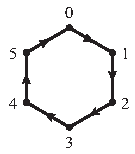
\includegraphics[width=\linewidth,height=.8\textheight,keepaspectratio]{assets/p090_00.pdf}\end{center}
\begin{center}\small\textbf{7.10 Figure}\end{center}\end{minipage}\hfill\begin{minipage}[t]{0.4903\linewidth}\vspace{0pt}\begin{center}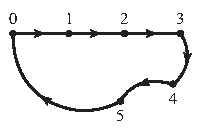
\includegraphics[width=\linewidth,height=.8\textheight,keepaspectratio]{assets/p090_02.pdf}\end{center}\end{minipage}
\end{center}
\end{BookFloat}

(a)

(b)

Two digraphs for \BookInline{\mathbb{Z}_{6}} with \BookInline{S= \{1\}} using

.

1

\begin{BookFloat}{07_generating_sets_and_cayley_digraphs-p90-6}
\begin{center}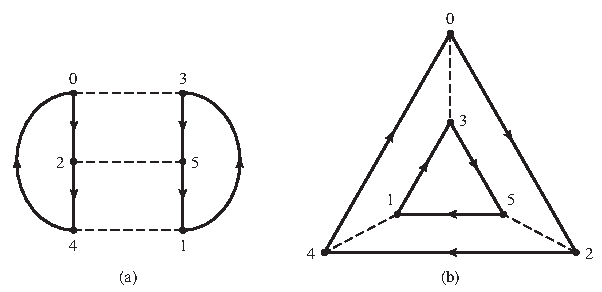
\includegraphics[width=0.826\linewidth,height=.8\textheight,keepaspectratio]{assets/review_v3_p090_7.11.pdf}\end{center}
\begin{center}\small \textbf{7.11 Figure}\quad Two digraphs for $\mathbb{Z}_6$ with $S=\{2,3\}$ using
\tikz[baseline=-.5ex]{\draw[->,thin] (0,0)--(12mm,0);\node[below=1pt,inner sep=0pt] at (6mm,0){\scriptsize $2$};}
and
\tikz[baseline=-.5ex]{\draw[->,thin,dashed] (0,0)--(12mm,0);\node[below=1pt,inner sep=0pt] at (6mm,0){\scriptsize $3$};}.\end{center}
\end{BookFloat}

\begin{BookFloat}{07_generating_sets_and_cayley_digraphs-p90-7}
\begin{center}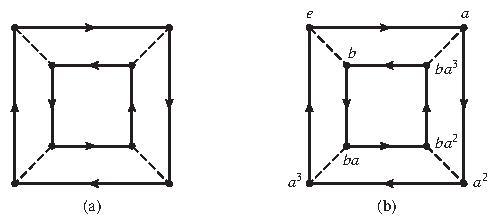
\includegraphics[width=0.680\linewidth,height=.8\textheight,keepaspectratio]{assets/review_v3_p090_7.13.pdf}\end{center}
\begin{center}\small \textbf{7.13 Figure}\end{center}
\end{BookFloat}

\BookTextHeading{\textit{\textbf{Property}}}

\BookTextHeading{\textit{\textbf{Reason}}}

1. The digraph is connected, that is, we can get from any vertex \BookInline{g} to any vertex \BookInline{h} by traveling along consecutive arcs, starting at \BookInline{g} and ending at \BookInline{h.}

Every equation \BookInline{gx= h} has a solution in a group.

2. At most one arc goes from a vertex \BookInline{g} to a vertex \BookInline{h.}

The solution of \BookInline{gx= h} is unique.

3. Each vertex \BookInline{g} has exactly one arc of each type starting at \BookInline{g,\allowbreak } and one of each type ending at \BookInline{g.}

For \BookInline{g\in G} and each generator \BookInline{b} we can compute \BookInline{gb,\allowbreak } and \BookInline{(gb^{- 1})b= g.}

4. If two different sequences of arc types starting from vertex \BookInline{g} lead to the same vertex \BookInline{h,\allowbreak } then those same sequences of arc types starting from any vertex \BookInline{u} will lead to the same vertex \BookInline{v.}

If \BookInline{gq= h} and\textit{ gr} \BookInline{= h,\allowbreak } then \BookInline{uq= } \BookInline{ug^{- 1}h= ur.}

\end{BookBody}

% Source PDF page 91; original printed page 74
\BookSource{91}{74}
\BookNarrativetrue

\begin{BookBody}

\noindent It can be shown that, conversely, every digraph satisfying these four properties is a Cayley digraph for some group. Due to the symmetry of such a digraph, we can choose labels like \BookInline{a,\allowbreak b,\allowbreak c} for the various arc types, name any vertex \BookInline{e} to represent the identity, and name each other vertex by a product of arc labels and their inverses that we can travel to attain that vertex starting from the one that we named \BookInline{e.} Some finite groups were first constructed (found) using digraphs.

\BookLabel{7.14 Example} A digraph satisfying the four properties given above is shown in Fig. 7.13 (a). To obtain Fig. 7.13 (b), we selected the labels

\begin{center}\begin{adjustbox}{max width=\linewidth}\BookInline{\displaystyle \xrightarrow{\quad\quad}\quad  and  \quad \xrightarrow{\quad\quad}\quad \xrightarrow{\quad\quad}}\end{adjustbox}\end{center}

\noindent named a vertex \BookInline{e,\allowbreak } and then named the other vertices as shown. We have a group

\begin{center}\begin{adjustbox}{max width=\linewidth}\BookInline{\displaystyle \{e,\allowbreak a,\allowbreak a^{2},\allowbreak a^{3},\allowbreak b,\allowbreak ba,\allowbreak ba^{2},\allowbreak ba^{3}\}}\end{adjustbox}\end{center}

\noindent of eight elements. From the diagram we could compute any product. For example, to compute \BookInline{ba^{2}ba^{3}} we start at the vertex labeled \BookInline{ba^{2},\allowbreak } follow a dotted edge, and then follow three solid edges to arrive at \BookInline{a.} Note that the way we labeled the vertices is not unique. For example, the vertex labeled \BookInline{ba^{3}} could have been labeled \BookInline{ab} simply by going along a different path starting at \BookInline{e.} This says that \BookInline{ab= ba^{3}.} We also see that \BookInline{a^{4}= e} and \BookInline{b^{2}= e.} We hope that this example is starting to look familiar. In fact, Figure 7.13 is a Cayley digraph of the dihedral group \BookInline{D_{4}.} We simply relabel \BookInline{a} with \BookInline{\rho } and \BookInline{b} with \BookInline{\mu }! \BookEnd{\blacktriangle}

\end{BookBody}

\BookNarrativefalse

\begin{BookBody}

\BookExerciseTitle{7}

\BookTextHeading{\textbf{Computations}}

\noindent In Exercises 1 through 8, list the elements of the subgroup generated by the given subset.

\BookExercise{1.}{The subset \BookInline{\{2,\allowbreak 3\}} of \BookInline{\mathbb{Z}_{12}}}

\BookExercise{2.}{The subset \BookInline{\{4,\allowbreak 6\}} of \BookInline{\mathbb{Z}_{12}}}

\BookExercise{3.}{The subset \BookInline{\{4,\allowbreak 6\}} in \BookInline{\mathbb{Z}_{25}}}

\BookExercise{4.}{The subset \BookInline{\{12,\allowbreak 30\}} of \BookInline{\mathbb{Z}_{36}}}

\BookExercise{5.}{The subset \BookInline{\{12,\allowbreak 42\}} of \BookInline{\mathbb{Z}}}

\BookExercise{6.}{The subset \BookInline{\{18,\allowbreak 24,\allowbreak 39\}} of \BookInline{\mathbb{Z}}}

\BookExercise{7.}{The subset \BookInline{\{\mu,\allowbreak \mu \rho ^{2}\}} in \BookInline{D_{8}}}

\BookExercise{8.}{The subset \BookInline{\{\rho ^{8},\allowbreak \rho ^{10}\}} in \BookInline{D_{18}}}

\BookExercise{9.}{Use the Cayley digraph in Figure 7.15 to compute these products. Note that the solid edges represent the generator \BookInline{a} and the dashed lines represent \BookInline{b.} \textbf{a}\BookInline{.(ba^{2})a^{3}} \textbf{b}\BookInline{.(ba)(ba^{3})} \textbf{c}\BookInline{.b(a^{2}b)}}

\begin{BookFloat}{07_generating_sets_and_cayley_digraphs-p91-18}
\begin{center}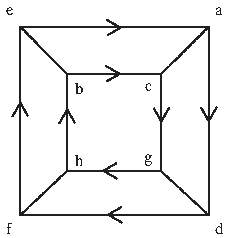
\includegraphics[width=0.312\linewidth,height=.8\textheight,keepaspectratio]{assets/p091_15.pdf}\end{center}
\begin{center}\small\textbf{7.15 Figure}\end{center}
\end{BookFloat}

\end{BookBody}

% Source PDF page 92; original printed page 75
\BookSource{92}{75}
\BookNarrativefalse

\begin{BookBody}

\noindent In Exercises 10 through 12, give the table for the group having the indicated digraph. In each digraph, take \BookInline{e} as identity element. List the identity \BookInline{e} first in your table, and list the remaining elements alphabetically, so that your answers will be easy to check.

\BookExercise{10.}{The digraph in Fig. 7.16(a)}

\BookExercise{11.}{The digraph in Fig. 7.16(b)}

\BookExercise{12.}{The digraph in Fig. 7.16(c)}

\begin{BookFloat}{07_generating_sets_and_cayley_digraphs-p92-4}
\begin{center}
\begin{minipage}[t]{0.2053\linewidth}\vspace{0pt}\begin{center}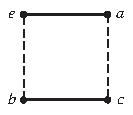
\includegraphics[width=\linewidth,height=.8\textheight,keepaspectratio]{assets/p092_04.pdf}\end{center}\end{minipage}\hfill\begin{minipage}[t]{0.2541\linewidth}\vspace{0pt}\begin{center}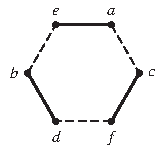
\includegraphics[width=\linewidth,height=.8\textheight,keepaspectratio]{assets/p092_06.pdf}\end{center}
\begin{center}\small\textbf{7.16 Figure}\end{center}\end{minipage}\hfill\begin{minipage}[t]{0.3659\linewidth}\vspace{0pt}\begin{center}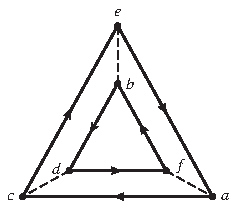
\includegraphics[width=\linewidth,height=.8\textheight,keepaspectratio]{assets/p092_09.pdf}\end{center}\end{minipage}
\end{center}
\end{BookFloat}

(a)

(b)

(c)

\BookTextHeading{\textbf{Concepts}}

\BookExercise{13.}{How can we tell from a Cayley digraph whether or not the corresponding group is commutative?}

\BookExercise{14.}{Using the condition found in Exercise 13, show that the group corresponding to the Cayley digraph in Figure 7.13 is not commutative.}

\BookExercise{15.}{Is it obvious from a Cayley digraph of a group whether or not the group is cyclic? [\textit{Hint:} Look at Fig. 7.9(b).]}

\BookExercise{16.}{The large outside triangle in Fig. 7.11(b) exhibits the cyclic subgroup \BookInline{\{0,\allowbreak 2,\allowbreak 4\}} of \BookInline{\mathbb{Z}_{6}.} Does the smaller inside triangle similarly exhibit a cyclic subgroup of \BookInline{\mathbb{Z}_{6}}? Why or why not?}

\BookExercise{17.}{The generating set \BookInline{S= \{1,\allowbreak 2\}} for \BookInline{\mathbb{Z}_{6}} contains more generators than necessary, since 1 is a generator for the group. Nevertheless, we can draw a Cayley digraph for \BookInline{\mathbb{Z}_{6}} with this generating set \BookInline{S.} Draw such a Cayley digraph.}

\BookExercise{18.}{Draw a Cayley digraph for \BookInline{\mathbb{Z}_{8}} with generating set \BookInline{S= \{2,\allowbreak 5\}.}}

\BookExercise{19.}{A\textbf{ relation} on a set \BookInline{S} of generators of a group \BookInline{G} is an equation that equates some product of generators and their inverses to the identity \BookInline{e} of \BookInline{G.} For example, if \BookInline{S= \{a,\allowbreak b\}} and \BookInline{G} is commutative so that \BookInline{ab= ba,\allowbreak } then one relation is \BookInline{aba^{- 1}b^{- 1}= e.} If, moreover\BookInline{,\allowbreak b} is its own inverse, then another relation is \BookInline{b^{2}= e.}}

\BookExercise{a.}{Explain how we can find some relations on \BookInline{S} from a Cayley digraph of \BookInline{G.}}

\BookExercise{b.}{Find three relations on the set \BookInline{S= \{a,\allowbreak b\}} of generators for the group described by Fig. 7.13(b).}

\BookExercise{20.}{Draw digraphs of the two possible structurally different groups of order 4, taking as small a generating set as possible in each case. You need not label vertices.}

\BookTextHeading{\textbf{Theory}}

\BookExercise{21.}{Use Cayley digraphs to show that for \BookInline{n\geq 3,\allowbreak } there exists a nonabelian group with \BookInline{2n} elements that is generated by two elements of order 2.}

\BookExercise{22.}{Prove that there are at least three different abelian groups of order 8. [Hint: Find a Cayley digraph for a group of order 8 having one generator of order 4 and another of order 2. Find a second Cayley digraph for a group of order 8 having three generators each with order 2.]}

\end{BookBody}
\ifdefined\BookMaster\let\BookFinish\relax\else\def\BookFinish{\end{document}}\fi\BookFinish
